
% \gr{
% TODO:
% \begin{itemize}
%     \item add link to github repos
%     \item  croissant file  
%     \item checklist 
%     \item\ [can be after deadline]upload to hugging face, upload to github repos, make nice readme on github 
% \end{itemize}
% }

\section{Introduction}
\looseness-1 Many real-world networks, such as social media networks~\cite{tgb}, human contact networks~\cite{shirzadkhani2024static} and financial transaction~\cite{shamsi2024graphpulse} networks can be formulated as temporal graphs or graphs that evolve over time. Recently, Temporal Graph Neural Networks (TGNNs) have emerged as promising architectures to address the unique challenges associated with ML on temporal graphs, which necessitates the modeling of both spatial and temporal dependencies~\citep{tgn, tgat, dygformer, skarding_tg_survey, ctan, feng_tg_survey}. Naturally, the development of TGNNs is quickly followed by an increased focus to design challenging benchmarks to understand their capabilities~\citep{poursafaei2022betterevaluationdynamiclink, tgb, tgb2.0, tgb-seq, shirzadkhani2024towards} across node, edge, and graph-level tasks. These benchmarks provide significant challenges for TGNNs in both scale and domain diversity with a focus on real-world tasks. However, current TGNNs have been shown to significantly struggle in these benchmarks and, in some cases, even underperform simple heuristics such as EdgeBank~\citep{poursafaei2022betterevaluationdynamiclink} and persistent forecast~\citep{tgb}.

\looseness-1 When compared to the increasing number of novel architectures proposed, exploring the weaknesses of TGNNs remains under-explored and often applies only to specific categories of methods~\citep{pint, weisfeiler-go-dynamic, tjandra2024enhancingexpressivitytemporalgraph, salzer2025logicalexpressivenesstemporalgnns}. \changed{Real-world benchmarks do not allow one to study TGNNs on temporal graph patterns in isolation}, and we argue that there is a strong need for a surgical and well-designed benchmark to highlight the weakness of existing models in performing crucial yet simple tasks on temporal graphs.

\looseness-1 In the past, diagnostic benchmarks were developed with different task classes to provide crucial insights into model capabilities precisely when complex, real-world benchmarks proved insufficient for pinpointing specific failure modes. For instance, in computer vision, the CLEVR dataset \citep{clevr} utilized synthetically generated scenes to test the compositional reasoning abilities of visual question-answering models, revealing limitations obscured by the biases and confounding factors present in natural images. Similarly, in early natural language processing, the bAbI dataset \citep{babi} provided a suite of 20 synthetic question-answering tasks generated algorithmically to probe basic reasoning skills (such as counting, induction, and deduction) essential for language understanding, offering metrics for progress on these core competencies. Reinforcement learning has also benefited from such focused evaluations; for instance, the Behaviour Suite for RL \citep{bsuite} includes controlled environments specifically designed to diagnose the memory and exploration capabilities of RL agents. 

\looseness-1 These examples demonstrate the power of purely synthetic datasets and environments designed for diagnostic evaluation: they allow for precise control over task complexity and the factors being tested, yielding clear insights into model strengths and weaknesses. Such a dedicated, synthetic diagnostic benchmark is currently missing for the domain of temporal graph learning (TGL). While existing benchmarks effectively test performance on complex, real-world dynamics, they inherently entangle various challenges, noisy interactions, complex graph structures evolving simultaneously with temporal patterns, and diverse event types. This makes it difficult to determine if a model's failure stems from an inability to handle graph complexity or from a fundamental deficit in capturing specific temporal patterns like periodicity, cause-and-effect relationships, or dependencies spanning long time horizons.

\looseness-1 To address this gap and facilitate a deeper, more interpretable understanding of TGNN limitations, we introduce the Temporal Graph Reasoning Benchmark (T-GRAB). \benchmarkname (\Cref{fig:tgrab}) comprises a suite of purely synthetic, \changed{discrete-time} temporal graph datasets explicitly designed to probe the fundamental temporal reasoning capabilities \changed{that we expect TGL models to exhibit}. By isolating core temporal patterns within controlled graph structures, \benchmarkname allows for a clear assessment of how well current TGNNs capture and generalize these patterns. 
\changed{By focusing on examining TGNNs basic reasoning capabilities on temporal graphs in a controlled environment, we show that even on simple synthetic graphs, models have difficulty capturing basic temporal structures}.


%\changed{(Comment 6) Our work introduces a series of experiments on small graphs to investigate whether TGNNs can capture simple temporal patterns and structures with a limited number of nodes, with scalability to larger graphs not being the primary focus of this study}.
% edit link
% https://drive.google.com/file/d/1_CL7XgYD36eWBMDmbSuSTJ_j2UhOYy4f/view?usp=sharing

\begin{figure*}[!t]
\vspace*{0.05cm}
    \centering
    % 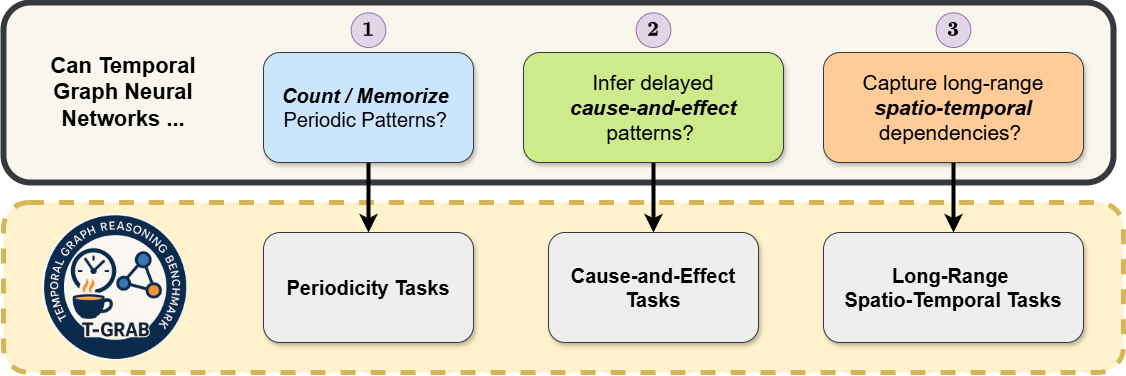
\includegraphics[width=\textwidth, keepaspectratio]{figs/T-GRABCrownV2.drawio.png}
    %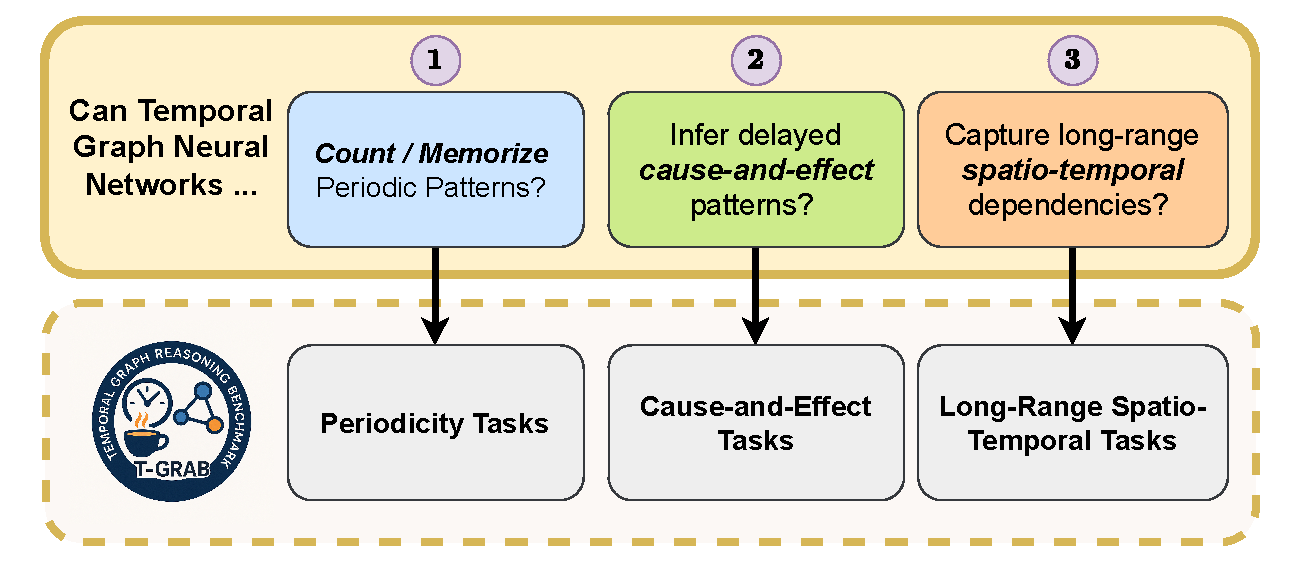
\includegraphics[width=0.7\textwidth, keepaspectratio]{kdd/figs/T-GRAB_flow.drawio.pdf}
    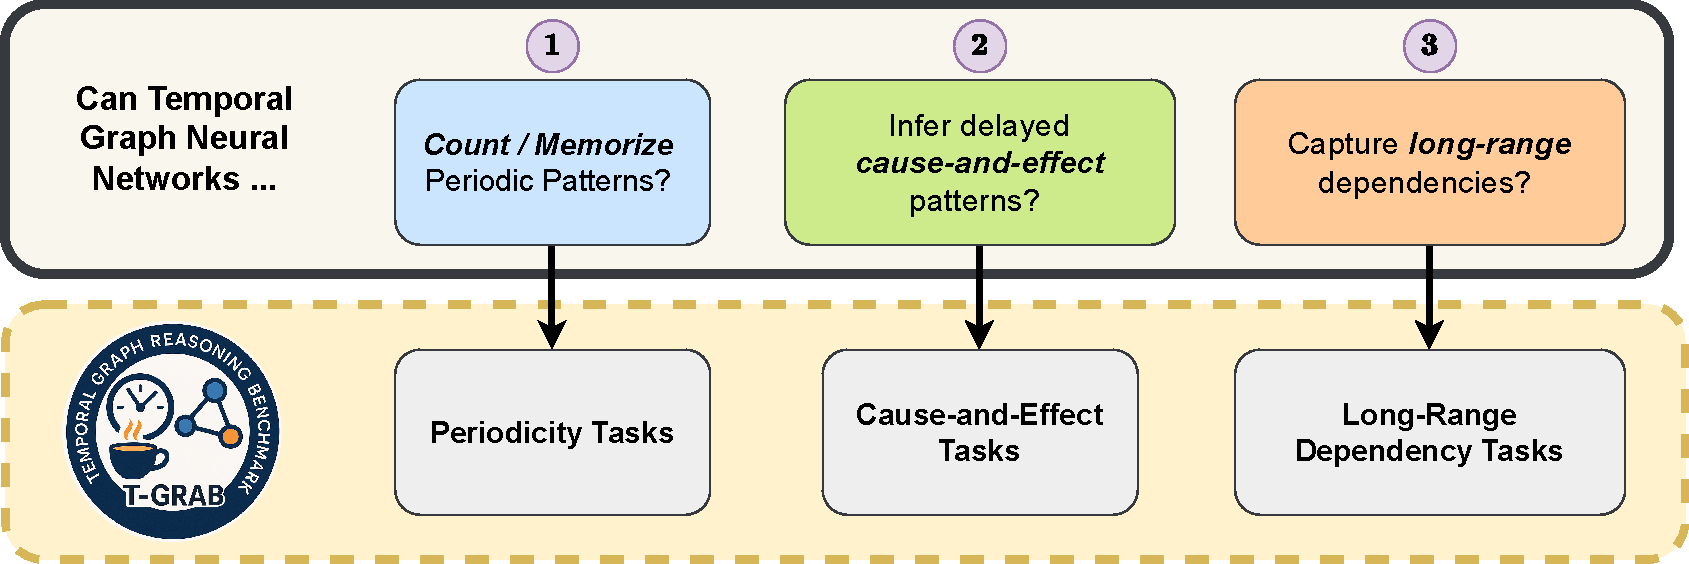
\includegraphics[width=0.7\linewidth, keepaspectratio]{kdd/figs/T-GRABCrownV2.pdf}
    % \caption{The questions T-GRAB asks and its associated tasks.}
    \caption{\benchmarkname is specifically designed to probe to which extent TGNNs exhibit fundamental basic reasoning skills over temporal graphs, including the abilities to: 1) recognize periodic structures, 2) capture delayed cause and effect relationships, and 3) reason across both temporal and spatial dimensions.   
    %tests the capabilities of TGNNs to reason over time in three fundamental aspects and includes three carefully designed tasks.
    }

     
     
    \label{fig:tgrab}
\end{figure*}

%(\Cref{fig:tgrab}) 

% \textbf{Contributions.} Our main contributions are as follows:
% \begin{itemize}[topsep=0pt]\itemsep0em 
%     \item To the best of our knowledge, \benchmarkname is the first synthetic dataset to systematically evaluate TGNNs’ temporal reasoning in a controlled setting. It includes three dynamic link prediction tasks: 1) \textbf{periodicity} to test \textit{counting/memorization}, 2) \textbf{cause-and-effect} to assess inference of \textit{delayed dependencies}, and 3) \textbf{long-range spatio-temporal} to evaluate \textit{spatial-temporal dependency modeling}. 
    
%     \item In the controlled environment of \benchmarkname, one can adjust the task difficulty to probe the limits of TGNNs, ultimately guiding the development of more robust and capable temporal graph learning methods. This additionally sheds light on the behaviors of TGNNs, which we observe are distinct between CTDG methods and DTDG methods. Further, from our experiments, we find that the number of temporal neighbors, a rarely modified hyperparameter, plays a significant role in model performance for \benchmarkname tasks.
    
%     \item For the periodicity tasks, GC-LSTM consistently performs best, even in the most challenging settings, indicating its recurrent structure is better suited for capturing periodic patterns and counting. In the cause-and-effect task, all models struggle with long-term memory, though DyGFormer, TGAT, and TGN degrade most gracefully. Finally, in the spatio-temporal task, DyGFormer's transformer-based architecture excels with short-range spatial dependencies, while TGAT and TGN outperform it as spatial dependencies grow longer.

%     \item All in all, there is no clear winner that performs best across all tasks, which differs from real-world benchmarks where a few top methods dominate the leaderboard. This shows that \benchmarkname can guide the design of future TGL methods which can strive to tackle all three tasks effectively. 

%     % We find that TGNNs struggle as task difficulty increases, shedding light on their underperformance in recent benchmarks. Notably, CTDG and DTDG methods show distinct behaviors, and the often-overlooked hyperparameter of temporal neighbors significantly impacts performance—especially in periodicity tasks.
%     % \item  \at{TODO: } how does our benchmark will help guide next steps for TGL method design benchmark will help to design robust method
    
%     % \item \benchmarkname provides a structured, controlled environment and evaluation framework that can expose current TGNNs' limitations and differentiates modeling strategies, ultimately guiding the development of more robust and capable temporal graph learning methods.

%  \end{itemize}


% [leftmargin=*] \itemsep0em 
\textbf{Contributions.} Our main contributions are as follows:
\begin{itemize} 
    \item We introduce T-GRAB, the first synthetic benchmark designed to systematically evaluate temporal reasoning capabilities of TGNNs \changed{ on fundamental temporal patterns in a controlled setting.} It features three carefully crafted temporal link prediction tasks: 1) \textbf{periodicity} to assess \textit{temporal pattern counting and memorization}, 2) \textbf{cause-and-effect} to evaluate \textit{delayed dependency inference}, and 3) \textbf{long-range dependency} to test \textit{long-range spatial and temporal dependencies}, i.e., structures involving nodes far away both in time and in the graph structure.
    
    \item \benchmarkname provides a configurable environment where task difficulty can be precisely adjusted to identify the limitations of TGNNs. Our experiments reveal distinct behavioral patterns between CTDG and DTDG methods, and highlight that the number of temporal neighbors, an often overlooked hyperparameter, significantly impacts model performance across our benchmark tasks.
    
     \item For the periodicity tasks, GC-LSTM consistently performs best, even in the most challenging settings, indicating its recurrent structure is better suited for capturing periodic patterns and counting. In the cause-and-effect task, all models struggle with long-term memory, though DyGFormer, TGAT, and TGN degrade most gracefully. Finally, in the long-range dependencies task, DyGFormer's transformer-based architecture excels with short-range spatial dependencies, while TGAT and TGN outperform it as spatial dependencies grow longer.

    
    \item Notably, no single model consistently outperforms across all tasks in T-GRAB, contrasting with real-world benchmarks where leaderboards are typically dominated by a few methods. This finding underscores the value of \benchmarkname as a diagnostic tool that can guide the development of more robust and versatile temporal graph learning methods capable of handling diverse temporal reasoning challenges.
\end{itemize}